\documentclass[a4paper,11pt,twoside]{report}
\usepackage[utf8]{inputenc}
\usepackage[top=2.5cm,bottom=2.5cm,outer=2.5cm,inner=2.0cm]{geometry}

\usepackage{amssymb}
\usepackage{amsmath}
\usepackage{booktabs}
\usepackage{hyperref}
\usepackage[noabbrev,capitalise]{cleveref}
\usepackage{colortbl}
\usepackage{color,soul}
\usepackage{xcolor}

\usepackage{enumitem}
% \setlist[enumerate,1]{label=\color{blue}(\arabic*)}
\setlist[enumerate,1]{label=(\arabic*)}

\usepackage{graphicx}
\usepackage{helvet}
\renewcommand{\familydefault}{\sfdefault}

\usepackage{hyperref}
\hypersetup{
	colorlinks = true,
	linkbordercolor = {white},
}

\usepackage{listings}

\usepackage{setspace}
\renewcommand{\baselinestretch}{1.3}

\usepackage{siunitx}
\usepackage{threeparttable}
\usepackage{multirow}

\begin{document}

\begin{center}
	{\large\textbf{NIMG-23-236: Responses to Editors and Reviewers}}
\end{center}

% Robin: cortex / brain stem / hippocampus /

% ========================================
%     Editor
% ========================================


% ========================================
%     Reviewer 1
% ========================================

\noindent \underline{\textbf{Reviewer 1}}

\textit{Authors propose an integrated acquisition and reconstruction methodology for accelerated multi-shell diffusion weighted imaging (DWI) based on an interleaved phase-encoding (PE) shifting and joint regularization with local low-rankness (LLR). The motivation is clear. The approach is original, although novelty is only incremental with respect to the state of the art. The methods are generally well presented, although certain details about the reconstruction algorithm are missing. The experimental section is weak, as quantitative comparisons or ablation/sensitivity analyses are missing, although the provided images illustrate the potential of the approach. The discussion is appropriate although some practically relevant points may be missing. The conclusions are generally well supported. Therefore, I would recommend a revision attending the points below.}

\vspace{1em}

\noindent \textit{Major:}

\begin{enumerate}
    \item \textit{No quantitative validation is provided. Authors should include quantitative comparisons of alternative methods using ground truth (GT) reconstructions (GT) built either from simulations or from retrospective subsampling of a long-enough DWI scan (or ideally from both).}

    \hspace{1em} Thank you for the suggestion.
    We acquired another dataset using 6-shot interleaved EPI
    and then retrospectively undersampled the data to only two shots.
    We compared the reconstructed DW images
    both qualitatively and quantitatively.
    Please refer to R1.1 in the annotated manuscript.

    \item \textit{Authors do not compare with JULEP, DAGER or SPA-LLR but these are cited as state of the art methods (more recent than MUSE and MUSSELS). Therefore, authors should also compare with these methods or else precisely indicate why are these left aside.}

    \hspace{1em} Thank you for the suggestion.
    We compared with MUSE, MUSSELS, and JULEP.
    We did not compare with DAGER
    because we did not have access to the source code.
    We did not compare with SPA-LLR because
    the SPA-LLR paper addresses the reconstruction problem
    of single-band acquisition.
    We thank all researchers who share their codes
    in the section Acknowledgments.

    \item \textit{For MUSSELS, authors should explicitly state if they base their implementation on Mani 2017 or Bilgic 2019 (whilst briefly motivating why). For local PCA, authors should more explicitly state whether they are comparing with Manjón 2013 or Veraart 2019.}

    \hspace{1em} We based our MUSSELS implementation on
    Bilgic 2019 (\href{https://doi.org/10.1002/mrm.27813}{10.1002/mrm.27813}) for two reasons.
    First, Dr.~Bilgic shares his MUSSELS implementation
    (see Acknowledgments).
    Second, Dr.~Bilgic's implementation allows for the reconstruction of
    multi-band multi-shot EPI data
    utilizing the readout extended FOV concept.

    \hspace{1em} For local PCA, we were computing with Manjón 2013.

    \item \textit{A sensitivity analysis based on the GT should be included considering these factors: LLR regularization weight, LLR block size, LLR overlap factor, PE interleave configuration (i.e., why 2 shots/b?). In case some of these factors are/need to be left aside, authors should precisely justify why. Ablation experiments comparing full proposal versus removing interleaved PE / removing LLR would also be very interesting.}
    \item \textit{LLR regularization performance and reliability may degrade in the presence of motion. Also, often DWI is performed with alternating PEs for distortion correction. SNR is heterogeneous over the FOV, which may not be appropriately covered by a single regularization weight. Please, add these aspects to discussion. See also minor point 5.}

    \hspace{1em} Thank you for the suggestion.
    We have incorporated motion into the discussion section.

    \item \textit{Abstract is focused on quite general motivating aspects, but paper methods and results are described in one/two sentences each. Authors should rebalance to provide abstract readers a better/quick understanding of paper content. Namely, shift-encoding and LRR ideas should be more clearly described in the abstract.}

    \hspace{1em} Thank you for the suggestion. We have clearly described
    in the abstract the ideas of shift encoding and LLR.

    \item \textit{Fig. 2 / Fig. 3 \textrightarrow you mention slice / diffusion direction included, but this is not very relevant, what matters is to specify the reasons for including these and not others. Also, it would be important to include snapshots at different slice locations within the brain, particularly at inferior locations, where reconstruction may become more challenging. Analogously, please provide rationale for snapshots selected in Fig. 4 and Fig. 5.}

    \item \textit{\url{https://github.com/ZhengguoTan/sigpy} seems a link to a generic tool. \url{https://doi.org/10.5281/zenodo.7548595} is not available yet. Please, remember to provide paper-specific links before acceptance or otherwise remove these links from the manuscript.}

    \hspace{1em} We forked sigpy (\url{https://github.com/mikgroup/sigpy}) for the development of
    our proposed reconstruction. We promise to publish our source codes in the forked sigpy.

    \hspace{1em} As shown in \cref{FIG:Zenodo},
    \url{https://doi.org/10.5281/zenodo.7548595} is a link we have already reserved
    to upload all raw data in this work upon the publication of our manuscript.
    Therefore, we would like to keep this link in the manuscript.

    \begin{figure}[ht]
        \centering
        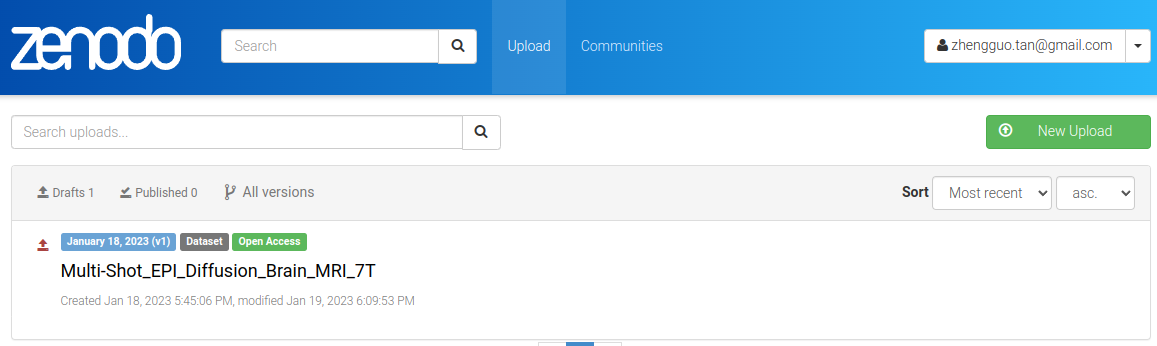
\includegraphics[width=\textwidth]{fig_zenodo.png}
        \caption{Reserved Zenodo link for the host of all raw data in this work.}
        \label{FIG:Zenodo}
    \end{figure}
\end{enumerate}


\noindent \textit{Minor:}

\begin{enumerate}[resume]
    \item \textit{Reference to 7T included in title does not seem relevant enough to me. Similar challenges for DWI can manifest for high resolution / high b-value lower field scans as well, so I'd recommend removing reference to 7T in title.}

    \hspace{1em} Since the primary aim of this work is
    to develop an efficient data sampling and image reconstruction technique
    for diffusion MRI at \SI{7}{\tesla}, we would like to keep \SI{7}{\tesla} in the title.

    \item \textit{L55: "DAGER requires many diffusion directions" \textrightarrow JETS also seems to require many diffusion directions, so guess this should be formulated differently?}

    We reformulated this paragraph.

    \item \textit{Section 2.2.1 and 2.2.2 \textrightarrow please, explicitly specify slice thickness.}

    \hspace{1em} Both protocols employ isotropic resolution.
    The slice thickness in Section 2.2.1 and 2.2.2 is \SI{1.2}{mm} and \SI{1.0}{mm}, respectively.

    \item \textit{L105: "acceleration" \textrightarrow would use "undersampling" as this is EPI and there's no 1-1 correspondence between undersampling and acceleration (several occurrences).}

    \hspace{1em} Done.

    \item \textit{L160: "As phase images are spatially smooth" \textrightarrow this may be arguable, would suggest replacing by "Assuming that phase images are spatially smooth". Think you should add a bit more on this topic to discussion, as phase behaviour depends on several hard-to-control factors such as pulsatile motion, its impact at different locations within the brain, diffusion sensitization strength, bulk motion,... so phase correction may sometimes be really challenging? Some additional lines of discussion on integration of navigators / cardiac gating could also be worthwhile.}

    \hspace{1em} Thank you for the suggestion.
    We have rephrased the sentence and added the topic of phase estimation to the discussion.

    \item \textit{L172: "firstly slides [...] matrices" \textrightarrow not very clear, think you should reword and explicitly mention what dimensions are concatenated in rows and columns of matrices. Also, reasons for not using 3D patches should be discussed.}
    \item \textit{L176: "$T^HT$ input neq input" \textrightarrow unclear, maybe a typo?}
    \item \textit{L181: "efficient implementation" \textrightarrow claim on efficiency does not seem supported from description... inverse density weighting is well-known for reconstructing original data levels back when slide-windowing. You should provide more details on efficiency or articulate description differently. Importantly, overlap ratio does not seem to be reported, but this may have a dramatic effect in computational cost.}
    \item \textit{Supporting Figure S3. "Small block size (i.e., 2) suffers from image blurring, whereas increasing block size gradually leads to increased noise" \textrightarrow may appear counter-intuitive as small block sizes should aid with localization and therefore prevent blurring, at the price of less information for denoising? Can you clarify on reasons / potential hidden factors for this behaviour?}
    \item \textit{L239: "blurring" \textrightarrow leading artifact resembles Rician bias rather than blurring in my opinion, could you clarify?}
    \item \textit{Seems Fig. 4 could be replaced by encompassing Supp. Fig. 6?}
\end{enumerate}


\noindent \textit{Typos, suggestions...}

\begin{enumerate}[resume]
    \item \textit{L33: "needed" \textrightarrow "used".}

    \hspace{1em} Done.

    \item \textit{L83: "benefits" \textrightarrow "benefits" to be stated experimentally, in methods better to refer to "properties"?}

    \hspace{1em} Done.

    \item \textit{L112: "as Section 2.2.1" \textrightarrow "as in Section 2.2.1".}

    \hspace{1em} Done.

    \item \textit{L119: "DW acquisition" \textrightarrow "DW acquisition volumes".}

    \hspace{1em} Done.

    \item \textit{L120: "demonstrates" \textrightarrow "will be used to demonstrate".}

    \hspace{1em} Done.

    \item \textit{L123: "slice collapsed k-space data" \textrightarrow not sure this expression is clear, you may consider rewording.}

    \item \textit{L125: "Such acquisition can be modeled in two ways." \textrightarrow "Acquisition modeling needs to consider several aspects.".}

    \hspace{1em} Done.

    \item \textit{L134: "at every" \textrightarrow "of each".}

    \hspace{1em} Done.

    \item \textit{L136: "shot images per" \textrightarrow "multiple shots acquired for a given".}

    \hspace{1em} Done.

    \item \textit{L137: "One method" \textrightarrow "A possibility".}

    \hspace{1em} Done.

    \item \textit{L141: "is done" \textrightarrow "can be done".}

    \hspace{1em} Done.

    \item \textit{L142: "This method can be written" \textrightarrow "This can be incorporated to our formulation".}

    \hspace{1em} Done.

    \item \textit{L147: "(e.g. Hanning window)" \textrightarrow would remove as there are many other possibilities, so this reference may not contribute to clarity of description?}

    \hspace{1em} Done.

    \item \textit{L148: "phase correction method" \textrightarrow "phase correction".}

    \hspace{1em} Done.

    \item \textit{L152: ", utilizing the concept of object-oriented linear operator abstraction" \textrightarrow not sure this is adding much, would remove.}

    \hspace{1em} Done.

    \item \textit{L168: "Intuitively, low rankness comes from contrast variation feature of DW images" \textrightarrow meaning unclear to me, you may reword.}

    \item \textit{L173: "patchs" \textrightarrow "patches".}

    \hspace{1em} Done.

    \item \textit{L176: "as an" \textrightarrow "as a".}

    \hspace{1em} Done.

    \item \textit{L185: "The acquired raw data was read by twixtools (URL)" \textrightarrow not adding much, could be specified in code repo.}

    \item \textit{L191: "the proximal operator" \textrightarrow "proximal operator".}

    \hspace{1em} Done.

    \item \textit{L196: "x E" \textrightarrow better to separate rather than concatenate description for both.}

    \hspace{1em} Done.

    \item \textit{L221: "GFA" \textrightarrow acronym does not seem defined.}

    \hspace{1em} Thank you. We added the definition.

    \item \textit{L247: "desnoing" \textrightarrow "denoising".}

    \hspace{1em} Done.

    \item \textit{L252: "within the rectangular regions in Fig. 4" \textrightarrow these may be difficult to appreciate, consider enhancing a bit perhaps?}


    \item \textit{L259: "smooth patterns" \textrightarrow "smoothness".}

    \hspace{1em} Done.

    \item \textit{L261: "spatial-angular" \textrightarrow really angular or b-vals are fused? Perhaps more accurate to say "spatial-diffusion"?}

    \hspace{1em} Done.

    \item \textit{L271: "achieves" \textrightarrow "uses".}

    \hspace{1em} Done.

\end{enumerate}


% ========================================
%     Reviewer 2
% ========================================
\clearpage
\noindent \underline{\textbf{Reviewer 2}}

\textit{This paper describes an image reconstruction method for diffusion-weighted segmented echo-planar imaging called JETS, which jointly processes all segments (shots) and diffusion weightings to explore local similarities between differently weighted images. This is achieved by adding a regularization term to the cost function guiding the image fitting that favors low-rankness of matrices created from image patches with different weightings. Additionally, inter-shot phase variations, which are a major problem of segmented diffusion MRI, are evaluated by separate pre-reconstructions of single segments and included in the signal model.\\
\indent Although the elements of the presented method have described before (low-rank modelling of image patches is used in SVD-filtering methods, and the single-shot phase mapping in MUSE, both duly cited), combining them in the reconstruction procedure is novel, and visibly provides superior results. The paper should meet the interest of MRI methodology-oriented readers even though the proposed strategy is not immediately applicable for routine scanning due to prohibitive computation times. I only have some minor remarks regarding the clarity of method description and the comparisons with established methods:}

\vspace{1em}

\begin{enumerate}
    \item \textit{It is not clear how the operator $T$ in Eq.~6 treats the multiple patches of the image. A graphical illustration of how the patches are combined to a 2D matrix whose nuclear norm is then taken would be helpful.}
    \item \textit{When the EPI segments are initially reconstructed to obtain the phase errors (Eq.~5), the related images surely represent single diffusion weighting. What is the T operator doing then in this equation? There is no diffusion dimension yet to impose a low rank approximation.}

    \hspace{1em} Very good question.

    \item \textit{How was the patch size and the overlap selected (on what basis)?}
    \item \textit{The proposed strategy involves a shift of the sampling pattern between diffusion weightings. The advantage of this shift is intuitively understandable, and it is reported as a result (lines 279-280) but not shown directly (comparisons with MUSE and MUSSELS involve more differences than the shift alone). It would be great to see the proposed joint reconstruction without the shift for comparison.}
    \item \textit{Is there any importance in the way the sampling shift is distributed among diffusion weightings?}

    \hspace{1em} In this work, multi-band and in-plane undersampled
    two-shot interleaved EPI was proposed.
    With in-plane undersampling,
    it is indeed important to have $k_y$ shifting.
    Please refer to \hl{Figure 3} in the manuscript.

    \item \textit{The proposed method seems very similar to MUSE with the PCA denoiser (the difference is that in JETS the LLR is promoted during the image fit, while in MUSE it is imposed afterwards) but delivers surprisingly better results. In the comparison of both strategies (Fig. 2) MUSE+PCA seems to reduce the noise stronger while some details are lost. If the PCA filter were made less aggressive, would MUSE still look worse than JETS?}
    \item \textit{In the same figure, MUSSELS shows similar details to JETS, but with more noise. Here, conversely, could not MUSSELS be improved by adding a moderate degree of PCA filtering?}
    \item \textit{The symbol $\mathcal{T}_{\lambda / \rho}$ is not defined in Eq.7.}

    \hspace{1em} Thank you. Defined.

\end{enumerate}



% ========================================
%     Reviewer 3
% ========================================
\clearpage
\noindent \underline{\textbf{Reviewer 3}}

\textit{The authors present a novel approach to accelerate diffusion imaging acquisitions by jointly reconstructing highly accelerated diffusion-weighted images recorded with different diffusion weightings and k-space sampling patterns. The underlying assumption is that by encoding complementary k-spaces in the different diffusion images, they can acquire a smaller k-space for each individual image, thus accelerating the overall acquisition. They show that their algorithm is able to reconstruct this undersampled data, whereas other contemporary reconstruction algorithms (which do not jointly reconstruct the data) perform less well.\\
\indent The principle is interesting, but I feel that the Authors are missing some important validation aspects, which are detailed as Major comments below.}

\vspace{1em}

\noindent \textit{Major comments}

\begin{enumerate}
    \item \textit{How many subjects were actually scanned? The Materials and Methods refers to "healthy volunteers", but I could not find an explicit number. The data presented in the paper seems to come from only a single subject. This is obviously inadequate to properly evaluate the performance of the method.}

    \hspace{1em} Three subjects were scanned in this work.

    \item \textit{Was there any correction for different eddy currents and motion between volumes? If not, why not? Eddy currents and (out-of-plane) motion could break the assumption that the low-rank patches reflect the same underlying anatomy. Perhaps the joint reconstruction method developed by the Authors actually mitigates these effects (and that would represent an additional advantage of the method), but correction would definitely need to be done in the case of the other reconstruction methods in order to make a fair comparison.\\
    As an aside, the Authors do refer to "motion robustness" several times, but this can surely only be robustness to in-plane motion. Out-of-plane motion in 2D imaging is harder as it is accompanied by a true loss of information. Model-based methods like that implemented in eddy (Andersson, et al. Neuroimage (2017) \url{https://doi.org/10.1016/j.neuroimage.2017.02.085}) can partially compensate for it, but don't seem to have been used here; and techniques like gSlider can correct for motion within the thick acquired slab during reconstruction (Wang, et al. Magn. Reson. Med. (2018) \url{https://doi.org/10.1002/mrm.27196}), but require specialised acquisitions.\\
    I would suggest that the Authors properly discuss the issues of eddy currents and intra- and inter-volume motion, and perhaps consider how they could properly incorporate a consideration of these effects into their framework.}
    \item \textit{Similarly to 2.: was there any correction for susceptibility distortions? I understand that the segmented EPI will have less distortions than conventional single shot EPI, but they still need to be corrected for to get anatomically correct images. Was the GRE scan perhaps used to make a B0 map which was included in the reconstruction?}
    \item \textit{It did not become clear to me why this study is being done at 7T. The increased sensitivity to B0 distortions and SNR loss with long TEs which this study proposes to overcome are 7T problems that are much less pronounced at 3T. In part it is for this reason that most DWI studies are still performed at 3T. What benefit are the Authors aiming to get from running DWI studies at 7T?}
    \item \textit{Relatedly, the acquisition scheme doesn't seem that fast. A similar scheme at 3T could even be shorter as T2 signal loss is less pronounced and so each (multiband) slice could be acquired in a single shot.}
    \item \textit{The denoising approach used as comparison does not reflect the state of the art. It is generally recommended to perform denoising on complex data (see Cordero-Grande, et al. Neuroimage (2019) \url{https://doi.org/10.1016/j.neuroimage.2019.06.039}), as this will avoid the noise floor issues that are apparent in the MUSE + Denoiser panel in Fig. 3. This should be completely possible for the Authors, as they reconstruct the data themselves. I would say the only reason not to do complex denoising at this point is if you are stuck with only scanner reconstructed magnitude data. Complex denoising is available in openly available toolboxes, e.g. MRtrix3 (\url{https://mrtrix.readthedocs.io/en/latest/reference/commands/dwidenoise.html}).}

    \hspace{1em} Thank you for the literature and the MRtrix tool.
    In fact, all reconstructions shown in this work were done off-line,
    including MUSE.
    We installed the MRtrix tool, and were able to use
    the denoising approach on complex MUSE images.

    \begin{figure}[ht]
        \centering
        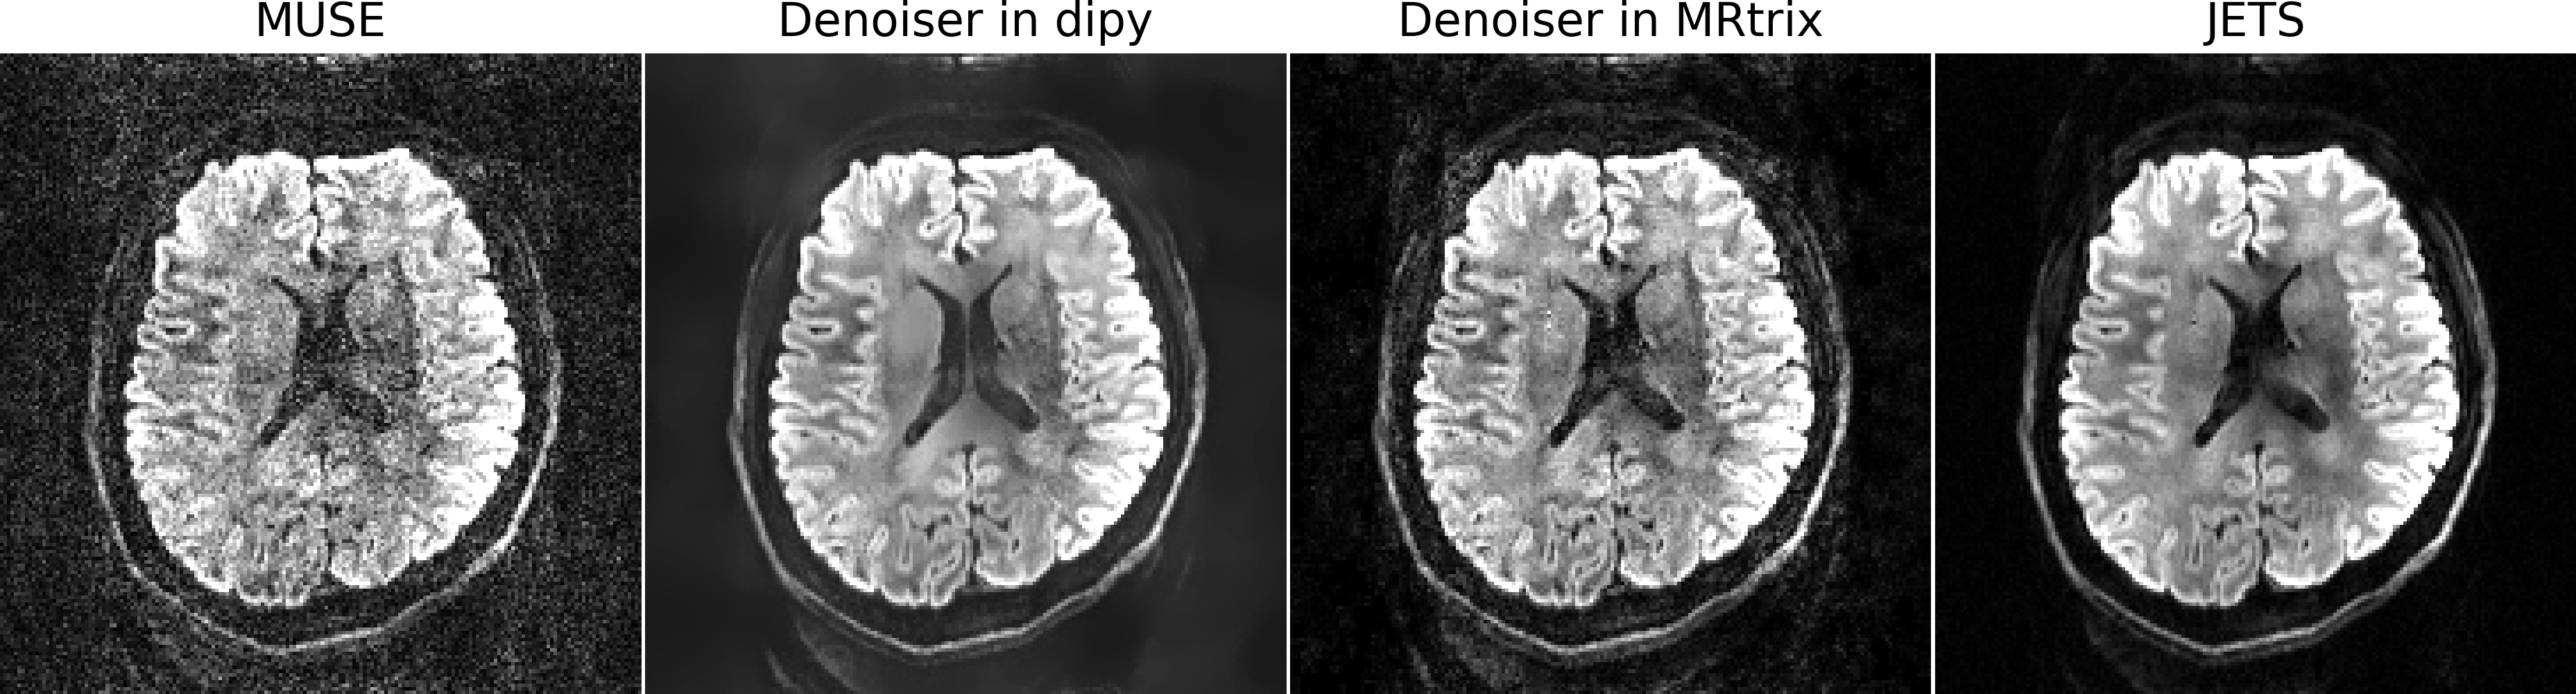
\includegraphics[width=\textwidth]{comp_dwi_denoiser.png}
        \caption{Comparison of one DW image
        (57th slice and 9th direction of
        the 1.2 mm isotropic resolution acquisition) from
        (1st column) MUSE,
        (2nd column) MUSE with the local-PCA denoiser in dipy,
        (3rd column) MUSE with the local-PCA denoiser on complex images in MRtrix, and
        (4th column) our proposed JETS reconstruction.}
        \label{FIG:Denoiser}
    \end{figure}

    As shown in \cref{FIG:Denoiser},

    \item \textit{While we are on the topic of "state of the art": All the papers in the Introduction demonstrating "conventional" SS-EPI are from over 20 years ago. There have been important technological developments, e.g. Connectom scanners, gradient inserts, sequence developments, e.g. multiband, gSlider, and image correction technique developments, e.g. the continued development of "topup" and "eddy", since then.}

    \hspace{1em} Thank you for the suggestion.
    We have included the techniques on multiband, gSlider, and topup
    in the Introduction.

    \item \textit{The Introduction is in general very confusingly written, and I would suggest considering how to put the introduced topics in a more logical order. As I see it, the fundamental problem is the trade-off between minimising distortions and maximising SNR while minimising acquisition time and sensitivity to motion, and this message does not come through clearly. For instance it is very confusing that it is suggested that navigators should be avoided because they increase the acquisition time, but segmented EPI -- which literally (at least) doubles the acquisition time while also introducing motion sensitivity -- is introduced as necessary without a consideration of the trade-offs.}

    \hspace{1em} Very good insights.
    We removed the statement on navigators in the Introduction.

    \item \textit{How were the number of directions in the three shell case determined? Generally 30 directions are recommended even for b = 1000 s/mm2, but here only 20 are used.}

    \hspace{1em} Thank you for the question.
    For the three-shell acquisition, we used the internal diffusion vector sets (DVS)
    available as the MDDW diffusion mode in Siemens scanners.
    The DVS with 20, 30, and 64 directions were used
    for the $b$-value of \num{1000}, \num{2000}, and \SI{3000}{s/mm^2},
    respectively.

    \item \textit{The "efficient implementation" to correct checkerboard artefacts (lines 177--183) seems very underspecified. Perhaps it would be better developed in an appendix and just mentioned in the main text? Specific points:}
        \begin{itemize}
            \item [-] \textit{is $(1/divisor)$ a matrix inverse of $(T'*T*1)$? Or is it rather a scalar derived by solving the linear equation $(T'*T*1) =$ (something)?}
            \item [-] \textit{is 1 the matrix of all ones, or the identity matrix?}
            \item [-] \textit{why would including this divisor prevent (or mitigate) checkerboard artefacts at all?}
        \end{itemize}
\end{enumerate}


\noindent \textit{Minor comments and typos}

\begin{enumerate}[resume]
    \item \textit{title should probably say "Diffusion *Weighted* Magnetic Resonance Imaging"}

    \hspace{1em} Done.

    \item \textit{typo in graphical abstract (METHODS (2): "reconsturction" instead of "reconstruction")}

    \hspace{1em} Thank you. Done.

\end{enumerate}


\noindent \textit{Abstract}

\begin{enumerate}[resume]
    \item \textit{high b-values do not "increase ... noise"; this should probably be rephrased to make clear that more strongly diffusion weighted images have lower SNR, thus increasing the *sensitivity to* noise.}

    \hspace{1em} Thank you. This has been rephrased.

    \item \textit{"inplane" should be "in-plane" for consistency with the rest of the document.}

    \hspace{1em} Done.

\end{enumerate}


\noindent \textit{Introduction}

\begin{enumerate}[resume]
    \item \textit{line 22: "spiral" is not a multi-shot EPI technique.}

    \hspace{1em} Thank you. We removed spiral here.

    \item \textit{line 37: should be "single shot images", not just "shot images"?}

    \hspace{1em} Thank you. Corrected.

    \item \textit{line 57: should be "in-plane".}

    \hspace{1em} Done.

    \item \textit{line 58: should be "still require long acquisition times".}

    \hspace{1em} Done.

    \item \textit{line 68: "i.e." should be "specifically".}

    \hspace{1em} Done.

    \item \textit{line 69: "the established DW image denoising algorithm, i.e., local PCA [REFS]" would be better written as "an established local PCA-based DW image denoising algorithm [REFS]" (though see the major comment above regarding whether this is state of the art).}

    \hspace{1em} Thank you. We rephrased this sentence.

\end{enumerate}


\noindent \textit{Materials and methods}

\begin{enumerate}[resume]
    \item \textit{line 73: should be "Materials and methods" (not "Material").}

    \hspace{1em} Done.

    \item \textit{line 92: the non-standard way of representing maximum gradient strength and slew rate should be written more explicitly.}

    \hspace{1em} Done.

    \item \textit{line 107: why are the b=0 images referred to as b = 50 $s/mm^2$ images here, but $b_0$ acquisitions for the three shell protocol? This should be standardised.}

    % TODO:

    \item \textit{line 107, 119: why is minutes$'$seconds$''$ notation used here but "min" elsewhere? Recommend standardising, especially since the used of minutes$'$seconds$''$ is fairly old-fashioned...}

    Thank you. Corrected.

    \item \textit{were the different b-values in the second acquisition scheme interleaved, or collected one after each other?}

    \hspace{1em}
    The different $b$-values were collected one after the other.
    In other words, we first acquired 20 diffusion encoding at the $b$-value of \SI{1000}{s/mm^2},
    then 32 diffusion encoding at the $b$-value of \SI{2000}{s/mm^2},
    and finally 64 diffusion encoding at the $b$-value of \SI{3000}{s/mm^2}.

    \item \textit{line 119: should be "acquisitions".}

    \hspace{1em} Done.

    \item \textit{line 139: presumably this should be "This method is robust to in-plane motion".}

    \hspace{1em} Thank you. Corrected.

    \item \textit{line 176: should be "a proximal operator".}

    \hspace{1em} Thank you. Corrected.

    \item \textit{line 177: "Noteworthy" is not usually used in this sense. Here it seems redundant and can be deleted.}

    \hspace{1em} Thank you. Deleted.

    \item \textit{line 180: I suggest "Hermitian adjoint" rather than just "adjoint".}

    \hspace{1em} Thank you. Added.

    \item \textit{line 183: should be "the input".}

    \hspace{1em} Thank you. Corrected.

    \item \textit{line 194: the meaning of the $\mathcal{T}$ symbol should be defined.}

    \hspace{1em} Done.

    \item \textit{line 196: again, "Noteworthy" is an odd choice here. I would suggest "Importantly".}

    \hspace{1em} Thank you. Replaced.

    \item \textit{line 196: missing "and" between "x E".}

    \hspace{1em} Thank you. Corrected.

    \item \textit{line 199: should be "conjugate gradients".}

    \hspace{1em} Thank you. Corrected.

    \item \textit{line 203: should be "as" not "ss".}

    \hspace{1em} Thank you. Corrected.

    \item \textit{line 206: NVIDIA seems to write the name of the GPU as "NVLink".}

    \hspace{1em} Thank you. Corrected.

    \item \textit{line 209: again, "i.e." should be "specifically".}

    \hspace{1em} Thank you. Corrected.

    \item \textit{line 212: "implemententation" should be "implementation" and quotes are backwards (should be ``).}

    \hspace{1em} Thank you. Corrected.

    \item \textit{lines 217--218: which shell or shells were used to compute the fODFs?}

    \hspace{1em} We used all shells to compute the fODFs.

    \item \textit{line 221: "GFA" abbreviation should be defined.}

    \hspace{1em} Defined.

\end{enumerate}


\noindent \textit{Results}

\begin{enumerate}[resume]
    \item \textit{line 228: should be "loses".}

    \hspace{1em} Thank you. Corrected.

    \item \textit{line 241: "allows to resolve" isn't a standard English construction. Should be something like "allows the resolution of".}

    \hspace{1em} Thank you. Corrected.

    \item \textit{line 247: should be "denoising".}

    \hspace{1em} Thank you. Corrected.

\end{enumerate}

\noindent \textit{Discussion}

\begin{enumerate}[resume]
    \item \textit{line 265: "dubbed as" is redundant; can just be "dubbed".}

    \hspace{1em} Done.

    \item \textit{line 273: should be "diffusion-directions".}

    \hspace{1em} We change to "per diffusion-weighted image".

    \item \textit{line 281: instead of "as" I would suggest "as used by".}

    \hspace{1em} Done.

    \item \textit{line 289: instead of "on GPU A100" I would suggest "on an A100 GPU".}

    \hspace{1em} Done.

    \item \textit{line 305: should be "solves for a fewer number of".}

    \hspace{1em} Done.

\end{enumerate}

\end{document}